\begin{frame}{Valgrind}
  \begin{columns}[T]
    \column{0.8\textwidth}
    \url{https://valgrind.org/}
    \begin{itemize}
    \item {\em instrumentation framework for building dynamic analysis tools}
      \begin{itemize}
      \item detect many memory management and threading bugs
      \item profile programs
      \end{itemize}
    \item Supported architectures: x86, x86-64, ARMv7, arm64, mips32,
      s390, ppc32 and ppc64
    \item Very popular tool especially for debugging memory issues
    \item Runs your program on a synthetic CPU $\rightarrow$
      significant performance impact (100 x slower on SAMA5D3!),
      but very detailed instrumentation
    \item Runs on the target. Easy to build with Yocto Project
	  or Buildroot.
    \end{itemize}
    \column{0.2\textwidth}
    
\includegraphics[width=\textwidth]{common/valgrind1.png}
  \end{columns}
\end{frame}

\begin{frame}{Valgrind tools}
  \begin{itemize}
  \item {\em Memcheck}: detects memory-management problems
  \item {\em Cachegrind}: cache profiler, detailed simulation of the
    I1, D1 and L2 caches in your CPU and so can accurately pinpoint
    the sources of cache misses in your code
  \item {\em Callgrind}: extension to Cachegrind, provides extra
    information about call graphs
  \item {\em Massif}: performs detailed heap profiling by taking
    regular snapshots of a program's heap
  \item {\em Helgrind}: thread debugger which finds data races in
    multithreaded programs. Looks for memory locations accessed by
    multiple threads without locking.
  \item More at \url{https://valgrind.org/info/tools.html}
  \end{itemize}
\end{frame}

\begin{frame}[fragile]{Valgrind examples}
  \begin{itemize}
  \item {\em Memcheck}
    \begin{block}{}
      {\tiny
\begin{verbatim}
$ valgrind --leak-check=yes <program>
  ==19182== Invalid write of size 4
  ==19182==    at 0x804838F: f (example.c:6)
  ==19182==    by 0x80483AB: main (example.c:11)
  ==19182==  Address 0x1BA45050 is 0 bytes after a block of size 40 alloc'd
  ==19182==    at 0x1B8FF5CD: malloc (vg_replace_malloc.c:130)
  ==19182==    by 0x8048385: f (example.c:5)
  ==19182==    by 0x80483AB: main (example.c:11)
\end{verbatim}
      }
    \end{block}

  \item {\em Callgrind}
    \begin{block}{}
      {\tiny
\begin{verbatim}
$ valgrind --tool=callgrind --dump-instr=yes --simulate-cache=yes --collect-jumps=yes <program>
$ ls callgrind.out.*
callgrind.out.1234
$ callgrind_annotate callgrind.out.1234
\end{verbatim}
      }
    \end{block}
  \end{itemize}
\end{frame}

\begin{frame}{Kcachegrind - Visualizing Valgrind profiling data}
  \begin{center}
    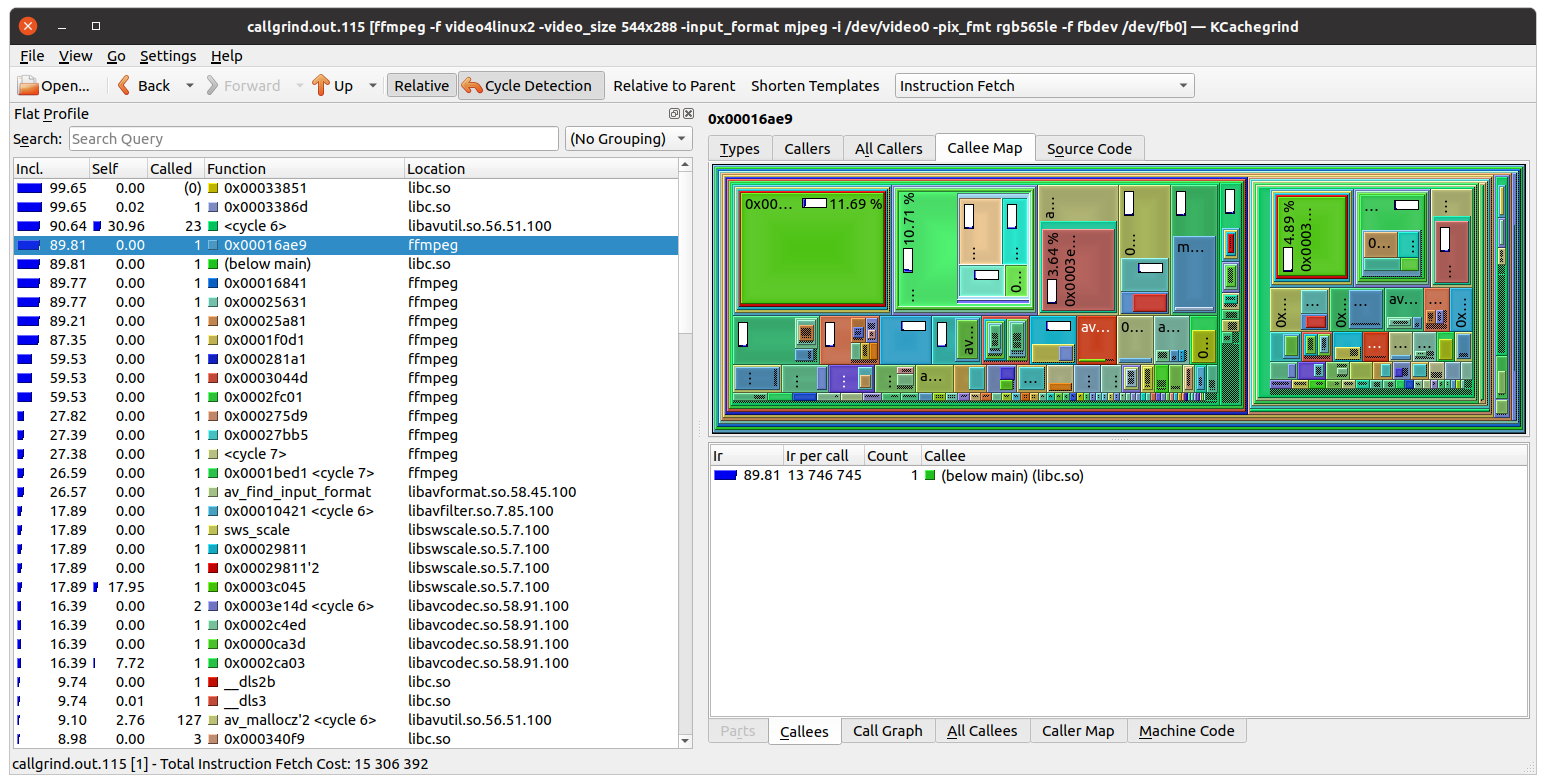
\includegraphics[height=0.8\textheight]{common/kcachegrind.png}
    \url{https://github.com/KDE/kcachegrind}
  \end{center}
\end{frame}
